\section{Domena czasowa}

Jednym ze sposobów analizy zmienności rytmu serca są metody z zakresu domeny czasowej,
które były stosowane historycznie najwcześniej. 
Wśrod nich można wyróżnić metody
badające cały szereg odstępów $RR$, powszechnie w literaturze przedmiotu oznaczającym
odległości $R$ lub inaczej czas pomiędzy kolejnymi załamkami w elektrokardiogramie.

Wielkości określające zmienność rytmu serca w tej domenie są stosunkowo najmniej
skomplikowane. Przykładowe zmienne to: średnia wartość interwału czy różnica pomiędzy
najdłuższym i najkrótszym odcinkiem. Jednakże ze względu na niestacjonarność szeregu $RR$
w naturalny sposób pojawia się konieczność wprowadzenia bardziej skomplikowanej analizy
statystycznej, na przykład wariancja zmiennej czasowej w całym lub w części nagrania.

W domenie czasowej możemy wyróżnić także innę grupę metod zwanymi metodami geometrycznymi.
Przymiotnik geometryczny wyraża fakt użycia obiektów geometrycznych jak np:
histogram rozkładu wartości $RR$ czy wykres \PP{} którego parametry reprezentują miarę HRV. 


\subsection{Analiza pełnej zmienności HRV}

Jednym ze sposobów analizy zmienności rytmu serca są metody z zakresu domeny czasowej,
które były stosowane historycznie najwcześniej. Wśrod nich można wyróżnić metody
badające cały szereg odstępów $RR$, powszechnie w literaturze przedmiotu oznaczającym
odległości $R$ lub inaczej czas pomiędzy kolejnymi załamkami w elektrokardiogramie.

Ze względu na użyty aparat matematyczny można wyróżnić tzw podejście wariancyjne w którym
powszechnie stosowanym parametrem jest parameter oznaczany jako $SDNN$ będący miarą pełnej
zmienności rytmu serca a wyrażony następującym wzorem:  

\begin{equation}\label{eq6}
SDNN = \sqrt{\frac{1}{n}\sum_{i=1}^{n}(RR_{i} - \overline{RR})^{2}}
\end{equation}

czyli jako pierwiastek z pełnej wariancji szeregu $RR$, gdzie $n$ jest to liczba odstępów $RR$
w całym nagraniu, $\overline{RR}$ oznacza zwykłą średnią, czyli:

\begin{equation}
\overline{RR} = \sum_{i=1}^{n}RR_{i}
\end{equation}

Nietrudno jest zauważyć że powyższe wyrażania odpowiadają drugiemu i pierwszemu momentowi
rozkładu dla szeregu odstępów $RR$. Sam w sobie szereg, wynika to także z natury
zjawiska jakim jest rytm serca, jest szeregiem niestacjonarnym w mocnym jak i słabym
sensie. Ten fakt oznacza że średnia jak i wariancja fluktuuje w czasie lub inaczej zmienia
się w zależności od tego który odcinek szeregu $RR$ analizujemy. W praktyce najcześciej
rozpatrywanymi długościami odcinka jest 5 lub 30 minut lub nagrania 24 godzinne.


\subsection{Deskryptory wykresu \PP{}}


Następna techniką z domeny czasowej wykorzystywaną do analizy HRV to technika opierająca
się na tzw. wykresach \PP{}.

Wykres \PP{}, którego nazwa pochodzi od twórcy tej techniki Henri \PP{}, jest\\ 
analityczno-wizualną technika ułatwiającą analizę złożonych zjawisk i ma ona zastosowanie
nie tylko w naukach medycznych ale także m.in. w meteorologii, geofizyce, astronomii.
Element wizualny wynika z użycia odpowiednio przygotowanych wykresów i w praktyce jest to
bardzo ważny element gdyż umożliwia na bardzo szybką wstępna jakościową analizę danego
zjawiska. Element analityczny jest związany z parametrami, tak zwanymi deskryptorami,
które wyrażają ilościowo informacje zawarte w wykresie \PP{}. Należy zaznaczyć że
metod ta jest bardzo odporna na dane zawierające artefakty lub wartości odstające i w
tym sensie ma przewagę nad technikami które wymagają niezakłóconych danych np 
wykorzystujące szybką transformatę Fouriera (FFT).

Konstrukcja wykresów \PP{} jest dość prosta, przyjmując że szereg $RR$ wyrazimy jako
wektor:
\begin{equation}
\bRR = (RR_{1}, RR_{2}, \ldots, RR_{n})
\end{equation}
oś odciętych jest utworzona z wektora $RR$ bez ostatniego elementu, natomiast oś rzędnych
zawiera elementy bezpośrednio po nich następujące, czyli wektor $RR$ bez elementu
pierwszego:
\begin{equation}
\bRRm = (RR_{1}, RR_{2}, \ldots, RR_{n-1}),
\bRRn = (RR_{2}, RR_{2}, \ldots, RR_{n}) 
\end{equation}
lub inaczej
\begin{equation}
  \mathcal{P} = \{(RR_1, RR_2),\ldots, (RR_i, RR_{i+1}), (RR_{n-1}, RR_n )\},
 \label{eq:p_plot}
\end{equation}
zatem wykres \PP{} jest zbiorem (chmurą) punktów $(RR_{i}, RR_{i+1})$ gdzie $i=(1, \ldots, n-1)$

Podstawowymi parametrami (deskryptorami) utworzonymi w oparciu o powyższą reprezentacją 
graficzną wektora $\bRR$ są parametry określane w literaturze symbolami $SD1$ i $SD2$, które
wyrażają odpowiednio zmienność krótko- i długoterminową rytmu serca.
%matematycznie wyrażonymi przy pomocy wariancji:

%\begin{equation}
%SD1^2 = Var\left(\frac{\bRRn - \bRRm}{\sqrt{2}}\right)
%\end{equation}

%\begin{equation}
%SD2^2 = Var\left(\frac{\bRRn + \bRRm}{\sqrt{2}}\right)
%\end{equation}

%Tak zdefiniowane~jak powyżej
Parametry $SD1$, $SD2$ mierzą rozproszenie punktów wykresu
\PP{} względem odpowiednio tzw linii identyczności $l_{I}$ (linii dla której $\bRRm = \bRRn$)
oraz linii prostopadłej do linii identyczności $l_2$ przechodzącej przez centroid. Na
rysunku \ref{fig:pp_distrib} została przedstawiona konstrukcja tych parametrów oraz zostały
przedstawione rzuty wariancji: histogram (a) krótkoterminowej zmienności rytmu serca $SD1$
wzdłuż linii identyczności $l_{I}$, histogram (b) pełnej zmienności rytmu serca na oś $RR_n$,
histogram (c) długoterminowej zmienności rytmu serca $SD2$ wzdłuż linii prostopadłej $l_2$
do linii identyczności $l_{I}$.

Jeśli zdefiniujemy szeregi różnic i sum współrzędnych punktów obróconego PP za pomocą
relacji:


\begin{equation}
\mathbf{L_1} = \left \{ \frac{RR_1 - RR_{2}}{\sqrt{2}}, \ldots, \frac{RR_i - RR_{i+1}}{\sqrt{2}}, \ldots, \frac{RR_{n-1} - RR_{n}}{\sqrt{2}} \right \},
\end{equation}
\begin{equation}
\mathbf{L_2} = \left \{\frac{RR_1 + RR_{2}}{\sqrt{2}}, \ldots, \frac{RR_i + RR_{i+1}}{\sqrt{2}}, \ldots, \frac{RR_{n-1} + RR_{n}}{\sqrt{2}} \right \},
\end{equation}
a~sam obrót jako:
\begin{equation}
\left[
    \begin{array}{c}
      x_i\\
      y_i\\
    \end{array} \right] 
  = 
\left[ \begin{array}{c c}
      \cos(\frac{\pi}{4}) & -\sin(\frac{\pi}{4})\\
      \sin(\frac{\pi}{4}) & \cos(\frac{\pi}{4})\\
    \end{array} \right] 
\left[
    \begin{array}{c}
      \mbox{RR}_i\\
      \mbox{RR}_{i+1}\\
    \end{array} \right],
\end{equation}
to parametry $SD1$ i $SD2$ możemy wyrazić jako wariancje szeregów $\mathbf{L_1}$ i $\mathbf{L_2}$ \cite{poinc_jaro,jarek2}:
\begin{equation}
  SD1^2 = \mbox{Var}( \mathbf{L_1})
  = \mbox{Var}\left(\frac{\bRRn - \bRRp}{\sqrt{2}}\right),
  \label{eq:sd1}
\end{equation}
\begin{equation}
  SD2^2 = \mbox{Var}( \mathbf{L_2})
  = \mbox{Var}\left(\frac{\bRRn + \bRRp}{\sqrt{2}}\right). 
  \label{eq:sd2}
\end{equation}

\begin{figure}
\centering
\includegraphics[width=\textwidth]{graph/pp_distrib.jpg}
\caption{Rysunek prezentuje położenie prostej równoległej ($l_1$) i~prostej prostopodłej ($l_2$) do osi identyczności separującej punkty reprezentujące skrócenia i~wydłużenia odstępów $RR$. Na wykresie przedstawiono również rozkłady punktów opisujących zmienność krótkoterminową $SD1$ (panel $a$ - rzut PP na oś $l_2$), zmienność długoterminową $SD2$ (panel $c$ reprezentujący rzut PP na oś $l_1$) oraz zmieność całkowitą (panel $b$ -- rzut PP na oś odciętych). Na histogramach różnymi odcieniami szarości oznaczono wkłady pochodzące od punktów, znajdujących się nad i~pod osią identyczności. Opracowano na podstawie \cite{hrstruct} -- rysunek udostępniony przez Jarosława Piskorskiego i~Przemysława Guzika na licencji CC BY.}
\label{fig:pp_distrib}
\end{figure}

Poniżej jeszcze inna postać na wariancje $SD1$ i $SD2$ tym razem oparta na własnościach geometrycznych linii identyczności występującej na rysunku \ref{fig:pp_distrib}: 

\begin{equation}
SD1^2 = \frac{1}{n}\sum_{i=1}^{n}r_{i}^{\perp 2}
\end{equation}

\begin{equation}
SD2^2 = \frac{1}{n}\sum_{i=1}^{n}r_{i}^{\parallel 2}
\end{equation}

gdzie $r_{i}^{\perp}$ jest prostopadłą odległością punktu $(RR_{i}, RR_{i+1})$ do linii
identyczności, $r_{i}^{\parallel}$ jest odległością punktu $(RR_{i}, RR_{i+1})$ do linii
$l_2$ wzdłuż linii identyczności.

Należy zaznaczyć że wyrażenie (\ref{eq:sd1}) dla krótkoterminowej zmienności rytmu serca
nie jest z matematycznego punktu widzenia odchyleniem standardowym, gdyż nie jest
wyznaczane względem linii $l_1$ przechodzącej przez centroid, to znaczy nie minimalizuje
drugiego momentu rozkładu punktów $RR$. Jednakże to w żaden sposób
nie umniejsza użyteczności tego deskryptora i to z dwóch powodów: (1) linia
identyczności dzieli cały wykres \PP{} na dwie części, górną dotyczącą zwolnień,
dolną dotyczącą przyspieszeń, zatem $SD1$ liczona względem $l_{I}$ ma wyraźną interpretację
fizjologiczną, (2) różnica pomiędzy wariancjami odnoszącymi się odpowiednio do linii $l_1$
oraz $l_{I}$ zgodnie z wartościami podanymi w \cite{poinc_jaro} jest rzędu $10^{-5}$ i
dąży do $0$ dla coraz większej liczby pomiarów, ponadto sam błąd związany z wprowadzeniem
wariancji względem $l_{I}$ jest rzędu $10^{-8}$, zatem w praktyce jest zaniedbywalny.

Relacja pomiędzy krótkoterminową i długoterminową zmiennością rytmu serca opisanymi powyżej
a miarą pełnej zmienności rytmu serca opisanej w \ref{subsec:pelna_zmiennosc}
jest następująca:
\begin{equation}
SDNN^2 = \frac{1}{2}(SD1^2 + SD2^2)\label{SDNNpartitioning}.
\end{equation}

\subsection{Deskryptory asymetrii rytmu serca}

Opierając się między innymi na analizie szeregów czasowych $RR$ przy pomocy wykresów \PP{}
grupa badaczy z Katedry i Kliniki Intensywnej Terapii Kadriologicznej i Chorób Wewnętrznych
Uniwersytetu Medycznego im. Karola Marcinkowskiego w Poznaniu oraz Instytutu Fizyki
Uniwersytetu Zielonogórskiego odkryła nowe zjawisko fizjologiczne w zmienności rytmu serca
nazwane asymetrią rytmu serca (ang. - Heart Rate Asymmetry - HRA). Słowo asymetria wyraża interesujące fenomen polegający na
tym, że wkład zwolnień rytmu serca w zmienności krótkoterminowej jest większy niż wkład
przyspieszeń \cite{guasym, biomed, geomasy,  berlinPrzemek,  annals, asym1, asym2,  asym3, asym4, asym5, asym6, asym7, car}, natomiast w zmienności długoterminowej i całkowitej odwrotnie, wkład
przyspieszeń jest większy niż wkład zwolnień \cite{guasym, berlinPrzemek,  annals}.

Elementem geometrycznym względem którego HRA jest definiowana to linia identyczności $l_{I}$ (rysunek \ref{fig:pp_distrib}). Linia identyczności jest jedyną linią posiadającą jasną interpretację fizjologiczną, dzieląca
rytm serca na grupy zwolnień i przyspieszeń.

Opierając się na właściwościach matematycznych wariancji można dokonać podziału wszystkich
parametrów wykresu \PP{}, tzn $SD1^2$, $SD2^2$ i $SDNN^2$, na części dotyczące zwolnień i 
przyspieszeń \cite{geomasy, annals, partitioning}.

\subsubsection{Deskryptory asymetrii krótkoterminowej}
Podział $SD1^2$ dla przyspieszeń i zwolnień wygląda następująco \cite{biomed, geomasy, annals, berlinJa}:
\begin{equation}
SD1^2=\frac{1}{n}\left(\sum_{i=1}^{n_{d}}[r^{\perp\;d}_{i}]^{2}+\sum_{j=1}^{n_{a}}[r^{\perp\;a}_{j}]^{2}\right),\label{SD1_podzial}
\end{equation}
gdzie:
\begin{enumerate}
\item[]$r^{\perp\;d}_{i}$ -- odległość prostopadła przyspieszającego punktu  wykresu \linebreak \PP{} o~indeksie $i$ do linii identyczności,
\item[]$r^{\perp\;a}_{j}$ -- odległość prostopadła zwalniającego punktu wykresu \PP\ o~indeksie $j$ do linii identyczności.
\end{enumerate}
oraz
\begin{enumerate}
\item[]$n_{d}$ -- jest liczbą zwolnień (punktów powyżej linii identyczności),
\item[]$n_{a}$ -- jest liczbą przyspieszeń (punktów poniżej linii identyczności).
\end{enumerate}
Faktycznie występuje jeszcze trzecia grupa punktów leżąca na linii identyczności, a zatem
$n$ będąca całkowitą ilością punktów bedzię zdefiniowana jako:
\begin{equation}
n=n_{d}+n_{a}+n_{on} \label{nki},
\end{equation}
jednakże punkty $n_{on}$ nie wnoszą żadnego wkładu do $SD1$, dlatego można je tutaj pominąć.

Wyrażenie (\ref{SD1_podzial}) składa się dwóch członów które w~naturalny sposób odpowiadają
wkładom zwolnień i~przyspieszeń w całkowitej $SD1^{2}$ 
\begin{equation}
SD1^{2}=SD1_{d}^{2}+SD1_{a}^{2}\label{SD1par},
\end{equation}
gdzie
\begin{equation}
SD1_{d}^{2}=\frac{1}{n}\sum_{i=1}^{n_{d}}[r^{\perp\;d}_{i}]^{2}, \qquad SD1_{a}^{2}=\frac{1}{n}\sum_{i=1}^{n_{a}}[r^{\perp\;a}_{i}]^{2}. \label{STpart}
\end{equation}
Do analizy porównawczej wariancje określone przez wzory (\ref{STpart}) użyte z danymi
pochodzącymi od różnych osób nie są zbyt pomocne, dlatego zostały wprowadzone wielkości
wyrażające znormalizowane wkłady zwolnień i przyspieszeń \cite{geomasy, annals, berlinJa}, tzn.:
\begin{equation}
C1_{d}=\frac{SD1_{d}^{2}}{SD1^{2}}, \qquad C1_{a}=\frac{SD1_{a}^{2}}{SD1^{2}},\label{STnorm}
\end{equation}
przy czym
\begin{equation}
C1_{d}+C1_{a}=1.
\end{equation}

\subsubsection{Deskryptory asymetrii długoterminowej}

Długoterminowa zmienność rytmu serca, $SD2$, obliczana jako wariancja względem linii
centroidu $l_2$ (rysunek \ref{fig:pp_distrib}), w przeciwieństwie do $SD1$, jest
najmniejszym możliwym drugim momentem w tym kierunku \cite{geomasy,annals,berlinJa}. Ponieważ, linia identyczności jest
jedyną linią z jasną interpretacją fizjologiczną to konstrukcja deskryptorów asymetrii dla
$SD2$ jest definiowana względem tej linii, natomiast linia $l_2$ prostopadła do linii
identyczności jest używana tylko do obliczeń.

Podział $SD2^2$ dla przyspieszeń i zwolnień jest koncepcyjnie bardzo podobny do wyrażenia
(\ref{SD1_podzial}), a mianowicie \cite{annals}
\begin{equation}
SD2^2= \frac{1}{n}\sum_{s=1}^{n}r^{||\;2}_{s}=\frac{1}{n}\left(\sum_{i=1}^{n_{d}}[r^{||\;d}_{i}]^{2}+\sum_{j=1}^{n_{a}}[r^{||\;a}_{j}]^{2}+\sum_{k=1}^{n_{on}}[r^{||\;on}_{k}]^{2}\right), \label{LTpart}
\end{equation}
gdzie:  
\begin{enumerate}
\item[]$r^{||}_{s}$ -- odległością punktu \emph{s} od $l_{2}$ wzdłuż linii identyczności,
\item[]$n_{d}$, $n_{a}$ i~$n_{on}$ -- są tak samo definiowane jak dla wzoru (\ref{SD1_podzial}), 
\item[]$r^{||\;d}_{i}$ -- odległość mierzona wzdłuż linii identyczności zwalniającego punktu  wykresu \PP\ o~indeksie $i$ do linii $l_{2}$,
\item[]$r^{||\;a}_{j}$ -- odległość mierzona wzdłuż linii identyczności przyspieszającego punktu  wykresu \PP\ o~indeksie $j$ do linii $l_{2}$.
\end{enumerate}
Podobnie jak w przypadku zmienności krótkoterminej, dwa pierwsze człony we wzorze (\ref{LTpart})
odpowiadają zwolnieniom i przyspieszeniom rytmu serca, jednakże to co odróżnia zmienność
długoterminową to niezaniedbywalny człon zawierający punkty na linii identyczności, czyli:
$1/n\sum_{k=1}^{n_{on}}[r^{||\;on}_{k}]^{2}$ w~(\ref{LTpart}). Wielkość członu związanego
z linią identyczności jest, jeśli tak można wyrazić, zależna sprzętowo, gdyż na ilość 
identycznych (co do wartości) sąsiadujących ze sobą punktów w szeregu $RR$ istotny wpływ ma
precyzja urządzenia pomiarowego. Czym większa precyzja, tym mniej punktów pomiarowych
wpada do tego samego przedziału pomiędzy dwoma dyskretnymi poziomami pomiarowymi, a to
znaczy dążenie do zera liczby punktów na linii identyczności \cite{annals}. 

W pracy \cite{annals} zaproponowano aby człon związany z linią identyczności miał
równy wkład, po połowie, do obu części zwolnień i przyspieszeń, i wielkości tak określone
okazują się bardziej konserwatywne, jak to pokazały testy statystyczne.
 
Podział asymetryczny dla zmienności długoterminowej $SD2$ definiuje się analogicznie jak w 
 (\ref{SD1par}), tzn.:
\begin{equation}
SD2^{2}=SD2_{d}^{2}+SD2_{a}^{2}, \label{SD2part}
\end{equation}
czyli na część pochodzącą od zwolnień i przyspieszeń, a odpowiednie wkłady do wariancji
przy pomocy następujących wyrażeń \cite{annals}:
\begin{eqnarray}
SD2_{d}^{2}&=&\frac{1}{n}\left(\sum_{i=1}^{n_{d}}[r^{||\;d}_{i}]^{2}+\frac{1}{2}\sum_{j=1}^{n_{on}}[r^{||\;on}_{j}]^{2}\right),\label{LTpartdef}\\
SD2_{a}^{2}&=&\frac{1}{n}\left(\sum_{i=1}^{n_{a}}[r^{||\;a}_{i}]^{2}+\frac{1}{2}\sum_{j=1}^{n_{on}}[r^{||\;on}_{j}]^{2}\right). \nonumber
\end{eqnarray}

Uwaga związana ze znormalizowanymi wkładami zwolnień i przyspieszeń przy okazji wzoru (\ref{STnorm})
obowiązuje także dla zmienności długoterminowej, co wyrażają następujące relacje:
\begin{equation}
C2_{d}=\frac{SD2_{d}^{2}}{SD2^{2}}, \qquad C2_{a}=\frac{SD2_{a}^{2}}{SD2^{2}},\label{LTnorm}
\end{equation}
gdzie
\begin{equation}
C2_{d}+C2_{a}=1.
\end{equation}

\subsubsection{Deskryptory asymetrii pełnej}
Opierając się na deskrytorach asymetrii krótko- i długoterminej można dokonać podziału
pełnej zmienności rytmu serca, wzór (\ref{SDNNpartitioning}), na składowe dla zwolnień i
przyspieszeń w następujący sposób \cite{annals}
\begin{eqnarray}
SDNN^{2}&=&\frac{1}{2}\left(\underbrace{(SD1_{d}^{2}+SD1_{a}^{2})}_{SD1^{2}}+\underbrace{(SD2_{d}^{2}+SD2_{a}^{2})}_{SD2^{2}}\right)\\
&=&\frac{1}{2}\left(\underbrace{(SD1_{d}^{2}+SD2_{d}^{2})}_{2SDNN_{d}^{2}}+\underbrace{(SD1_{a}^{2}+SD2_{a}^{2})}_{2 SDNN_{a}^{2}}\right).\nonumber
\end{eqnarray}
lub inaczej jako
\begin{equation}
SDNN^{2}=SDNN_{d}^{2}+SDNN_{a}^{2}, \label{SDNNpart}
\end{equation}
przy czym 
\begin{equation}
SDNN_{d}^2=\frac{1}{2}\left(SD1_{d}^{2}+SD2_{d}^{2}\right),\quad SDNN_{a}^2=\frac{1}{2}\left(SD1_{a}^{2}+SD2_{a}^{2}\right). \label{SDNNpartad}
\end{equation}

Wyrażenie (\ref{SDNNpartad}) w naturalny sposób umożliwia zdefiniowanie	znormalizowanych
wkładów zwolnień i przyspieszeń do pełnej zmienności rytmu serca \cite{annals}
\begin{equation}
C_{d}= \frac{SDNN_{d}^{2}}{SDNN^{2}},\qquad C_{a}= \frac{SDNN_{a}^{2}}{SDNN^{2}}\label{SDNNcontrib}.
\end{equation}
przy czym
\begin{equation}
C_{d}+C_{a}=1.
\end{equation}

Proces konstruowania deskryptorów asymetrii krótko- i długoterminowej jest zobrazowany na
rysunku~\ref{habfig2_2}{.}

Zgodnie z analizą przeprowadzoną w \cite{geomasy,annals} asymetria krótkoterminowa w grupie $N$
badanych osób zachodzi w stopniu istotnym statystyczne, jeśli: 
\begin{equation}
C1_{d}>C1_{a},
\end{equation} 
Natomiast asymetria długoterminowa zachodzi w stopniu istotnym statystycznie \cite{annals}, jeśli:
\begin{equation}
C2_{d}<C2_{a},
\end{equation}
oraz asymetria całkowita jest określona gdy w~grupie $N$ badanych osób, jeśli jest
spełniona poniższej nierówność w stopniu istotny statystycznie \cite{annals}
\begin{equation}
C_{d}<C_{a}.
\end{equation}
Wielkość próby oraz szczegóły metod statystycznych użytych w celu określenia zachodzenia
powyższych warunków zostały podane w pracy \cite{geomasy}.

\subsubsection{Aplikacje kliniczne deskryptorów asymetrii}

Opierając się na danych klinicznych, jak to zostało pokazane w pracach \cite{guasym, biomed, geomasy, annals} 
potwierdzono występowanie asymetrii krótkoterminowej w szeregach odstępów $RR$ u osób 
zdrowych w spoczynku i to w stopniu wysoce istotnie statystycznym. Podobnie, asymetria
długoterminowa została potwierdzona w grupie osób zdrowych w spoczynku w stopniu wysoce
istotnie statystycznym, w pracach \cite{guasym, annals}. Także w tych pracach została potwierdzona
asymetria rytmu serca względem pełnej zmienności rytmu serca, $SDNN^2$, w stopniu wysoce
istotnie statystycznym. Natomiast w pracach \cite{berlinPrzemek, asym1, asym2, asym4, car} można znaleść kliniczne aplikacje
wariancyjnych parametrów asymetrii rytmu serca.

Ponieważ opisane w tym rozdziale deskrytory asymetrii są ze swojej natury pojęciami
całkowicie ogólnymi, mogą być użyte także do badanie asymetrii innych zjawisk medycznych.
I tak, w pracy \cite{hypertension_asym}, została zbadana (i potwierdzona) asymetria krótkoterminowa w zmienności
sygnału ciśnienia tętniczego. Stwierdzono, że jest ona niezależna od HRA.
%\linebreak %przeniesienie związane ze składem
\begin{landscape}
\begin{figure}
\begin{center}
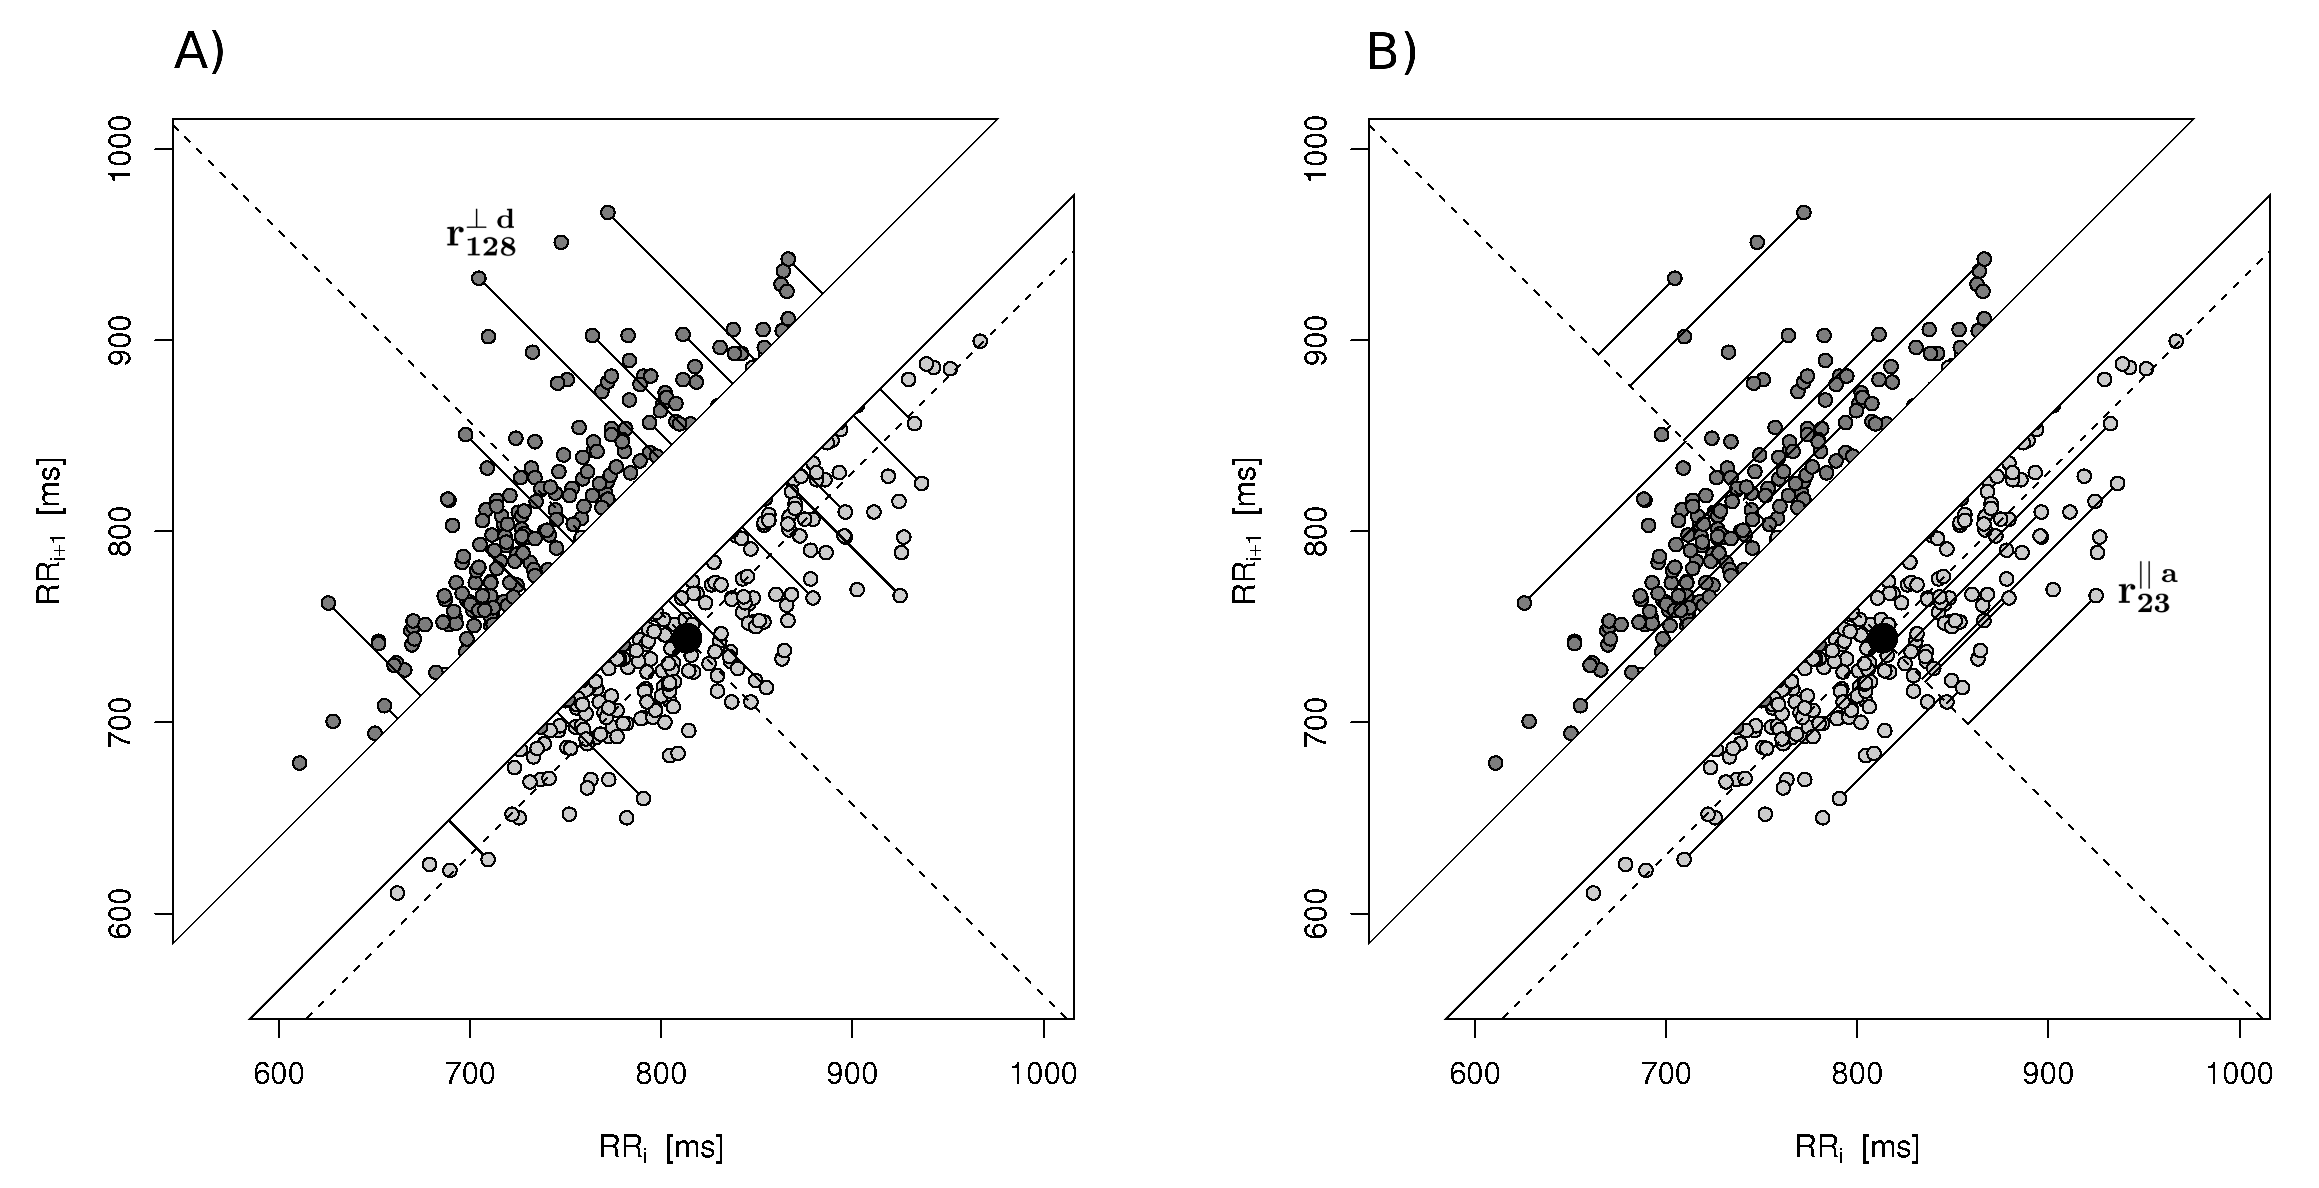
\includegraphics[width=1.5\textwidth]{graph/habfig2_2a}
\caption{W panelu A) przedstawiono konstrukcję deskryptorów krótkoterminowej HRA, a~w~panelu B) proces konstrukcji deskryptorów długoterminowej HRA. Należy zwrócić uwagę, że linia identyczności jest najistotniejszym obiektem geometrycznym w~obu konstrukcjach -- jest ona jedynym kryterium decydującym o~tym, czy dany punkt wnosi wkład do części wariancji ($SD1^2$, $SD2^2$ lub $SDNN^2$) związanej ze zwolnieniami czy przyspieszeniami. $r^{\perp\;d}_{128}$ jest prostopadłą odległością (zwalniającego) punktu wykresu \PP{} numer $128$ do linii identyczności, $r^{||\;a}_{23}$ jest prostopadłą odległością (przyspieszającego) punktu numer $23$ od linii $l_{2}$.\label{habfig2_2}}
\end{center}
\end{figure}
\end{landscape}
\clearpage
